\section{Primeira Arquitetura Customizada}

\subsection{Aplicação}

Como o foco do trabalho não é no desenvolvimento em si, mas sim nas práticas Devops que auxiliam o build, deploy e operação de uma aplicação em produção, foi utilizada uma aplicação fictícia baseada em um projeto de código aberto. O projeto será uma loja virtual sobra a plataforma Broadleaf Commerce 

\url {(http://www.broadleafcommerce.org/)}. 

O projeto pode ser acessado no seguinte repositório do Github: 

\url {http://github.com/dtsato/loja-virtual/devops/}

Serão utilizados as funcionalidades padrão de um site de compras online como Submarino ou a Amazon:

\begin{itemize}

\item Navegação e busca no catálogo de \item produtos;
\item Páginas de produto com nome, descrição, preço, fotos e produtos relacionados;
\item Carrinho de compras;
\item Processo de checkout customizável incluindo códigos promocionais, dados de cobrança e de entrega;
\item Cadastro de usuário;
\item Histórico de compras;
\item Ferramentas de administração para: catálogo de produtos, promoções, preços, taxas de frete e páginas com conteúdo customizado


\end{itemize}

\begin {figure} [!htb]
\centering
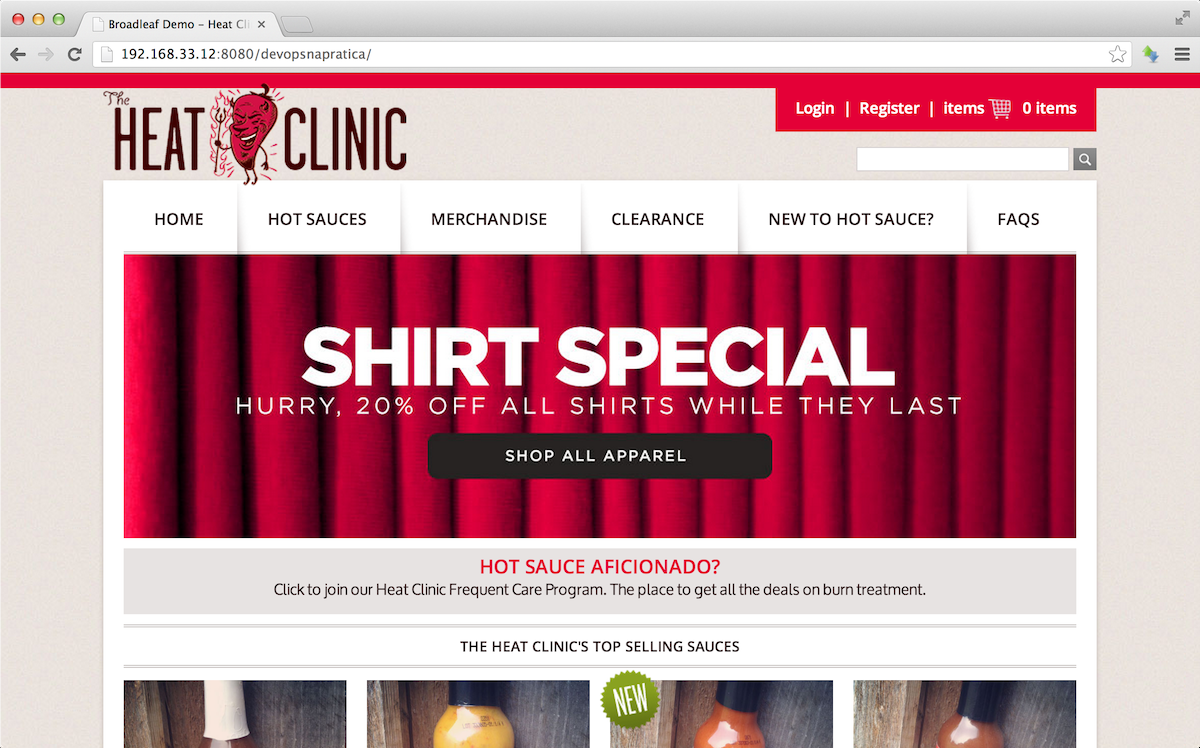
\includegraphics[scale=0.5]{imagens/label_loja}
\caption{Uma prévia da da página inicial da loja virtual}

\end{figure}

As tecnologias utilizadas na aplicação da loja virtual foram:

\begin{itemize}

\item \textbf{Java:} a aplicação e escrita em Java(\url{http://java.oracle.com/}) , compatível
com a versão Java SE 6 e superiores.

\item \textbf{Spring:}o Spring (\url{http://www.springframework.org/}) e um framework
de desenvolvimento de aplicações corporativas popular na comunidade
Java que oferece diversos componentes como: injeção de dependências,
gerenciamento de transações, segurança, um framework de MVC, dentre
outros.

\item \textbf{JPA e Hibernate:} o JPA e a API de persistência do Java e o Hibernate
(\url{http://www.hibernate.org/}) e a implementação mais famosa da
JPA na comunidade Java, oferecendo recursos para realizar o mapeamento
objeto-relacional (object-relational mapping ou ORM) entre objetos
Java e as tabelas no banco de dados.

\item \textbf{Google Web Toolkit:} o GWT (\url{http://developers.google.com/web-toolkit/}) e um framework desenvolvido pelo Google para facilitar
a criação de interfaces ricas que rodam no browser. O GWT permite
que o desenvolvedor escreva código Java que e então compilado para
Javascript. A loja virtual utiliza o GWT para implementar a interface
gráfica das ferramentas de administração.

\item \textbf{Apache Solr:} o Solr (\url{http://lucene.apache.org/solr/)} e um servidor de
pesquisa que permite a indexacao do catalogo de produtos da loja virtual
e ofereceuma API eficiente e flexivel para efetuar consultas de texto
em todo o catalogo.

\item \textbf{Tomcat:} o Tomcat (\url{http://tomcat.apache.org/}) e um servidor que implementa
as tecnologias web  Java Servlet e JavaServer Pages  do Java
EE. Apesar do Broadleaf Commerce rodar em servidores de aplicação
alternativos  como Jetty, GlassFish ou JBoss  utilizaremos o Tomcat
por ser uma escolha comum em diversas empresas rodando aplicações
web Java.

\end{itemize}

\subsection{Ambiente de Produção}

Usuários acessarão a loja virtual em uma instância do Tomcat no servidor web. O servidor web rodará todas as bibliotecas e frameworks Java utilizados pela loja virtual, inclusive uma instância embutida do Solr. Por fim, a aplicação web utilizará o MySQL, rodando em um servidor de banco de dados separado. Esta é uma arquitetura web de duas camadas comumente utilizada por diversas aplicações no mundo real.

\begin {figure} [!htb]
\centering
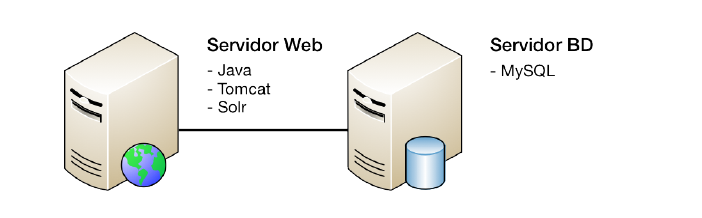
\includegraphics{imagens/servidores}
\caption{Ambiente de produção da loja virtual}
\end{figure}

Será utilizado a ferramenta VirtualBox para instanciação dos dois servidores chamados no presente trabalho de servidor web   e servidor bd em um ambiente Linux Ubuntu 12.04 LTS de 32 bits.
Para gerenciamento da dos dois servidores foi utilizado o Vagrant. O Vagrant é uma ferramenta para o building completo em ambientes de desenvolvimento.
O Vagrant file foi configurado da seguinte forma:

\begin {figure} [!htb]
\centering
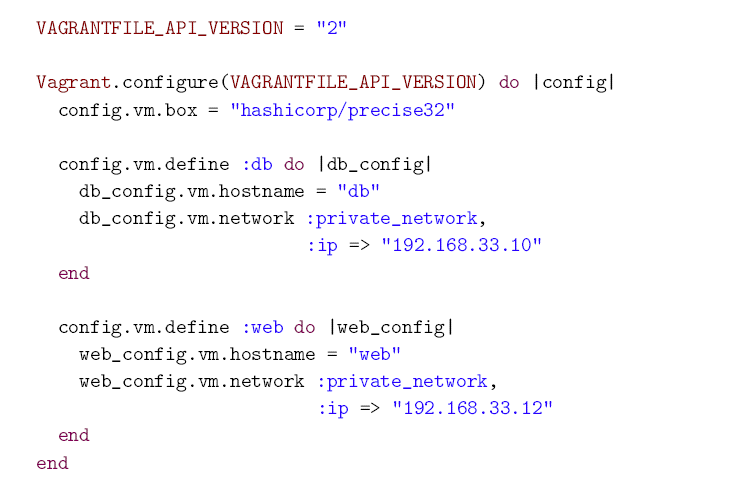
\includegraphics{imagens/vagrantfile}
\caption{Configuração declarada no VagrantFile}
\end{figure}

\subsection{Build e Deploy da Aplicação}

Nessa etapa será baixado e compilado o código, rodar os testes, empacotar a aplicação e colocar a loja virtual no ar. Esse processo de compilação, teste e empacotamento é conhecido como build. As etapas do processo de build também podem incluir gerenciamento de dependências, rodar ferramentas de análise estática do código, cobertura de código, geração de documentação, dentre outros. A principal função do processo de build é gerar um ou mais artefatos, com versões específicas, que se tornam potenciais candidatos para release  em produção.
Para realizar o build foi preciso instalar as seguinte ferramentas:

\begin{itemize}

\item Git (\url{http://git-scm.com}) para controle de versão
\item Maven (\url{http://maven.apache.org/}) para executar o build 
\item JDK (Java Development Kit) para compilação do código Java

\end{itemize}


As etapas na primeira execução do Maven serão:


\begin{itemize}

\item \textbf{Sub-projetos:}o projeto esta organizado em 4 módulos: core possui
as configurações principais, extensões e customizações da loja virtual;
site e a aplicação web da loja virtual; admin e uma aplicação web
restrita para administração e gerenciamento da loja virtual; por fim,
combined e um modulo que agrega as duas aplicações web e o core
em um único artefato. Cada modulo atua como um subprojeto que o
Maven precisa realizar o build separadamente.

\item \textbf{Resolução de dependências:}  o Maven ira resolver todas as dependências
do projeto e baixar as bibliotecas e frameworks necessários para
compilar e rodar cada modulo da loja virtual.

\item \textbf {Compilação:} o código Java e GWT precisa ser compilado para execução.
Isso toma um bom tempo na primeira vez. O compilador Java e
inteligente o suficiente para recompilar apenas o necessário em builds
subsequentes.

\item \textbf {Testes automatizados:} em módulos que definem testes automatizados,
o Maven ira executa-los e gerar relatórios de quais testes passaram e
quais falharam.

\item \textbf {Empacotamento de artefatos:} por fim, o modulo core será empacotado
Como um arquivo .jar enquanto os módulos web ( site, admin
e combined) serão empacotados como um arquivo .war. Ambos os
arquivos jar e war são equivalentes a arquivos zip que você baixa
regularmente da internet, no entanto a estrutura interna dos pacotes e
bem definida e padronizada pelo Java: o jar contém classes compiladas
e serve como biblioteca enquanto o war contém classes, bibliotecas,
arquivos estáticos e de configuração necessários para rodar uma
aplicação web em um container Java como o Tomcat.

\end{itemize}


As etapas futuras para o projeto serão:

\begin{itemize}

\item Configuração e implementação de um Servidor de Monitoramento utilizando o Nagios (\url{http://www.nagios.org/}). 

\item Configuração de ferramenta de gerenciamento de configurações para automatizar o processo de provisionamento, configuração e deploy da loja virtual utilizando o Puppet.

\item Configuração e estabelecimento de um sistema de controle de versões utilizando o Git (\url{http://git-scm.com/})

\item Configuração e estabelecimento do provisionamento do repositório de pacotes utilizando o Reprero (\url{http://mirrorer.alioth.debian.org/})

\item Realização de Deploy na Nuvem

\end{itemize}

